\section{Generalized Linear Models}
\label{sec:linear}

Our first attempts to identify at-risk students come from applying several variants of Generalized Linear Models.  Given some subset of the feature classes, we build a linear model of how binge drinking varies with the input variables and use that to form predictions for novel data.

\subsection{Algorithms}

In this section we explore four different algorithms based on Generalized Linear Models.  Here we use a single linear term corresponding to each input feature; see section 4.3 for a discussion of incorporating interaction terms.  The four algorithms are as follows:

\begin{enumerate}
\item \emph{Constant} - This extremely simple algorithm does not take the input features into account at all, and instead always predicts the most common class (no binge drinking in the past 2 weeks) as shown in Table \ref{C1}.  It serves as a lower bound on classification performance.
\item \emph{GLM - Gaussian} - We use R's built-in glm() function \cite{glm} to model the category of binge drinking as a linear function of the input features, assuming a Gaussian error distribution on the response variable.  We model our categorical response as numerical by giving each category a number from 1 to 6 in increasing order, so 1 is ``none'' and 6 is ``10+ times''.  This predicts a real-valued response; we achieve better accuracy with some postprocessing.  Namely, the real-valued predictions are clamped to the range 1 to 6 and rounded to an integer, since the correct response will always be integral.  Empirically we found that the best rounding method is almost always to round down - this encodes our knowledge that most people are not likely to engage in binge drinking.
\item \emph{GLM - Poisson} - This is the same as the \emph{GLM - Gaussian} algorithm except that the response variable is modelled with a Poisson error distribution.  The same postprocessing techniques are applied here, but using a Poisson distribution intuitively models the survey response data better than a Gaussian.
\item \emph{Ordered Logistic Regression} - Finally, we use the lmr() function from R package \emph{rms} \cite{lrm} to perform ordered logistic regression, often also known as ordered logit.  This captures the fact that the response variable is ordinal - the responses are divided into discrete categories, but the categories are not wholly independent as there is a clear ordering relationship between them.  Given a new student's features, we find the probability that they fall into each category of binge drinking and predict the one with the highest probability.
\end{enumerate}

\begin{figure}[t]
\centering
\makebox[\textwidth][c]{
\subfigure[]{
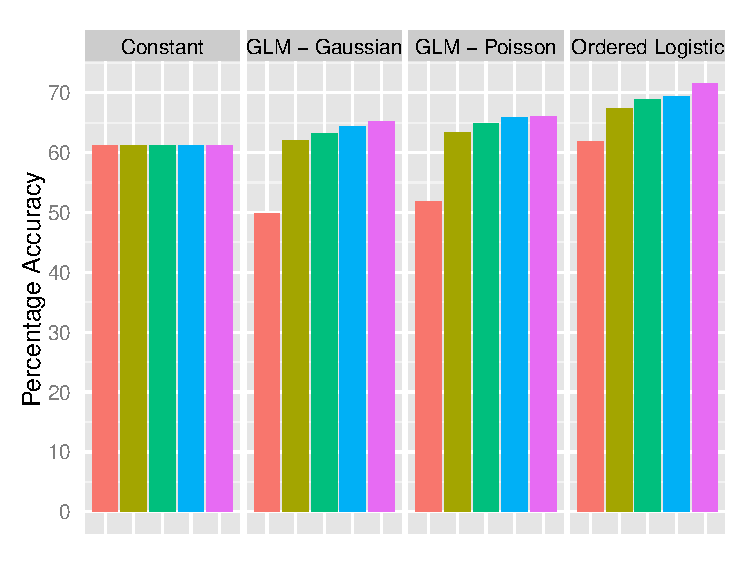
\includegraphics[scale=0.65]{linear_percent.pdf}
\label{linear_percent}
}
\subfigure[]{
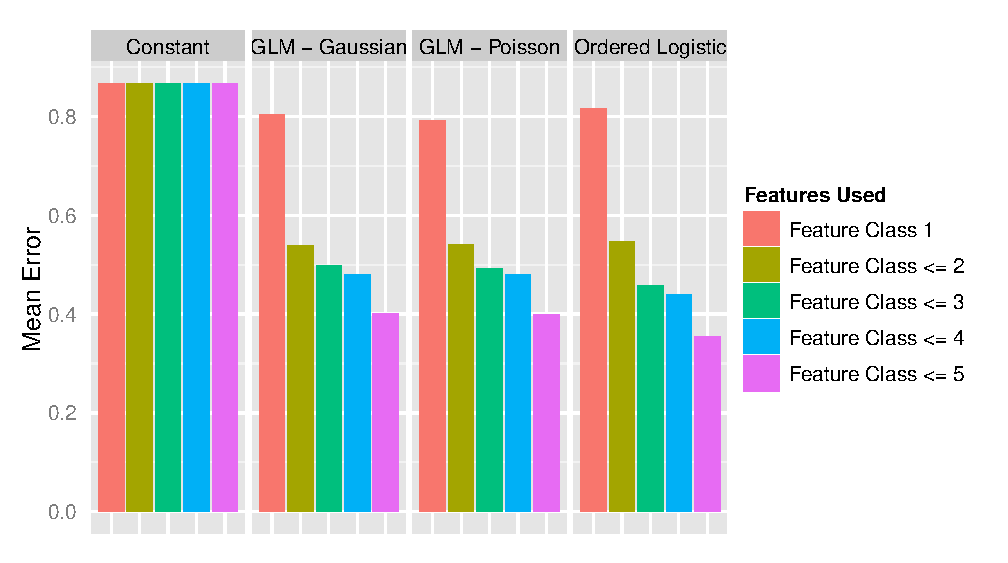
\includegraphics[scale=0.65]{linear_error.pdf}
\label{linear_error}
}
}
\caption{Predictive accuracy and mean error of each algorithm using various feature classes.}
\label{linear_results}
\end{figure}

\subsection{Results}

Figure \ref{linear_results} summarizes the performance of the four algorithms using 5-fold cross validation on our training/testing dataset.  As defined earlier, Figure \ref{linear_results} \subref{linear_percent} shows the percent accuracy metric and Figure \ref{linear_results} \subref{linear_error} shows the mean error.  The Constant algorithm which does not take the data into account at all achieves an accuracy of 61.2\% and a mean error of 0.867.  This gives an upper bound on the mean error we should expect to see, as all other algorithms achieve a strictly better mean error regardless of what features are available.  In terms of predictive accuracy, though, both versions of GLM actually do worse than Constant when only class 1 features are used.  The best performance comes from Ordered Logistic Regression when all features are available, with a percentage accuracy of 71.6\% and a mean error of 0.354.

The two versions of GLM perform extremely similarly on the whole, with Poisson slightly outperforming Gaussian in most cases - this is not unexpected given the true format of the response variable.  Interestingly, when only feature classes 1 and 2 are available, Ordered Logistic Regression actually has a slightly higher mean error than both versions of GLM.  Its percentage accuracy, on the other hand, is still much better in these cases, reminding us that the two evaluation metrics capture subtle differences in algorithmic performance.  Once class 3 or above features are available, though, Ordered Logistic Regression becomes the clear winner with the highest percentage accuracy and lowest mean error.

\subsection{Extensions}

There are several possible extensions to the algorithms used here that may lead to better predictive performance.  Surprisingly, however, the ones that we tried did not lead to any improvements.  Incorporating first-order interaction terms complicated the model and greatly increased the runtime of our experiments but did not increase the percentage accuracy or decrease the mean error.  To make the linear model simpler, we tried reducing the number of terms by building the model incrementally, using the Akaike information criterion \cite{} to decide which linear and interaction terms to add.  Again, this was much more computationally expensive than the basic models but performed no better.  Finally, we also tried regularized regression in the form of LASSO \cite{LASSO}.  Full results are omitted for brevity, but while LASSO's basic predictions were better than our GLM algorithms at some values of the regularization parameter, it seemed to interact poorly with the rounding/flooring technique we use to convert the predictions to a categorical variable.  Further investigations on this front may yield improvements, however.
